\section{Hardware}
In this chapter, we give a short oversight what hardware is used and how big the price tag of the demonstrator is. 

\subsection{Computer}
The computer used is the Nvidia Jetson Nano developer kit.
A short technical overview is listed in Table \ref{development:nano}.
\begin{table}[ht]
	\begin{tabular}{|l|l|}
		\hline
		\multicolumn{2}{|c|}{Technical specifications of the Jetson Nano} \\
		\hline
		GPU			& 	128-core Maxwell\\
		CPU			& 	Quad-core ARM A57 @ 1.43 GHz \\
		Memory 		&	4 GB 64-bit LPDDR4 25.6 GB/s 				\\
		Storage		&	microSD				\\
		Video Encode&	4K @ 30 | 4x 1080p @ 30 | 9x 720p @ 30 (H.264/H.265) \\
		Video Decode&	4K @ 60 | 2x 4K @ 30 | 8x 1080p @ 30 | 18x 720p @ 30 (H.264/H.265) \\
		Camera 		&	2x MIPI CSI-2 DPHY lanes \\
		Connectivity&	Gigabit Ethernet, M.2 Key E\\
		Display 	&	HDMI and display port \\
		USB 		&	4x USB 3.0, USB 2.0 Micro-B\\
		Others 		&	GPIO, I2C, I2S, SPI, UART \\
		Mechanical 	&	69 mm x 45 mm, 260-pin edge connector \\		
		\hline
	\end{tabular}
	\caption{Jetson Nano specifications \cite{jetson}.\label{development:nano}}
\end{table}

\newpage
\subsection{Camera}
The camera used for this project had to following evaluation criteria to meet:
\begin{itemize}
	\item Compatible with the Jetson Nano enviroment
	\item A good developer community
	\item Open source drivers
	\item Low cost
\end{itemize}

Table \ref{development:cameras} lists some of the cameras that have been evaluated for the project.
\begin{table}[ht]
	\centering
	\begin{tabular}{ |l||c|c|c|  }
		\hline
		\multicolumn{4}{|c|}{List of possible Cameras} \\
		\hline\hline
		Company				& Raspberry Pi 		& Raspberry Pi	& Arducam\\
		Camera Name			& Camera Module V2 	& HQ Camera		& Arducam IMX219 \\
		&					&				&Low Distortion M12 \\
		&					&				&Mount Camera Module\\
		\hline
		Price				& \$25 				& \$50  		& \$39.99 \\
		Camera Sensor   	& Sony IMX219 		& Sony IMX477	& Sony IMX219\\
		
		Still resolution	& 8M 				& 12M			& 12.3M\\
		Sensor resolution 	& 3280 x 2464 		& 4056 x 3040 	& 3280 x 2464\\
		Linux integration   & V4L2 driver 		& V4L2 driver	& V4L2 driver\\
		Pixel size			& 1.12 x 1.12 $\mu\text{m}$	& 1.55 x 1.55$\mu\text{m}$ & 1.12 x 1.12 $\mu\text{m}$ \\
		Focal length		& 3.04$[\text{mm}]$ & Depends on lens & 2.8$[\text{mm}]$\\
		Focal ratio			& 2.0  				& Depends on lens & 2.8\\
		View angle Horizontal & 62.2 deg.		& Depends on lens & 75 deg.\\
		\hline
	\end{tabular}
\caption{List of suitable cameras.\label{development:cameras}}	
\end{table}

In the end, all results were measured with the Raspberry Pi Camera Module V2 since it was the cheapest one in the list and seems to deliver the desired results.

\subsection{Backlight}
The main component of the backlight is a PCB.
In front of the PCB there are three stacked glass plates, on which diffusion filters and the geometry pattern later used for the measurements can be attached.
This is shown in Figure \ref{development:glass}.
\begin{figure}[ht]
	\centering
	\setlength{\tabcolsep}{12em}
	{\renewcommand{\arraystretch}{1}	
	\begin{tabular}{|c|}
		\hline
		\multicolumn{1}{|c|}{glass (2\,mm)}\\
		\hline
		\multicolumn{1}{|c|}{geometry pattern}\\
		\hline
		\multicolumn{1}{|c|}{glass (2\,mm)}\\
		\hline
		\multicolumn{1}{|c|}{diffusion filter}\\
		\hline
		\multicolumn{1}{|c|}{glass (2\,mm)}\\
		\hline
	\end{tabular}
	}
	\caption{Stacked glass plates.\label{development:glass}}
\end{figure}

The geometry pattern consists of five black squares in two rows.
The PCB is equipped with 39 LEDs and used two times.
One LED has a luminious flux of 76\,lm @ 4000\,K 80\,CRI \cite{led}.
The backlight should therefore have a total luminious flux of 5928\,lm.
The whole backlight consumes ca. 12\,A at 5\,V, which corresponds to a total power consumption of 60\,W. 

The PCB is shown in Figure \ref{development:pcb}.
\begin{figure}[ht]
	\centering
	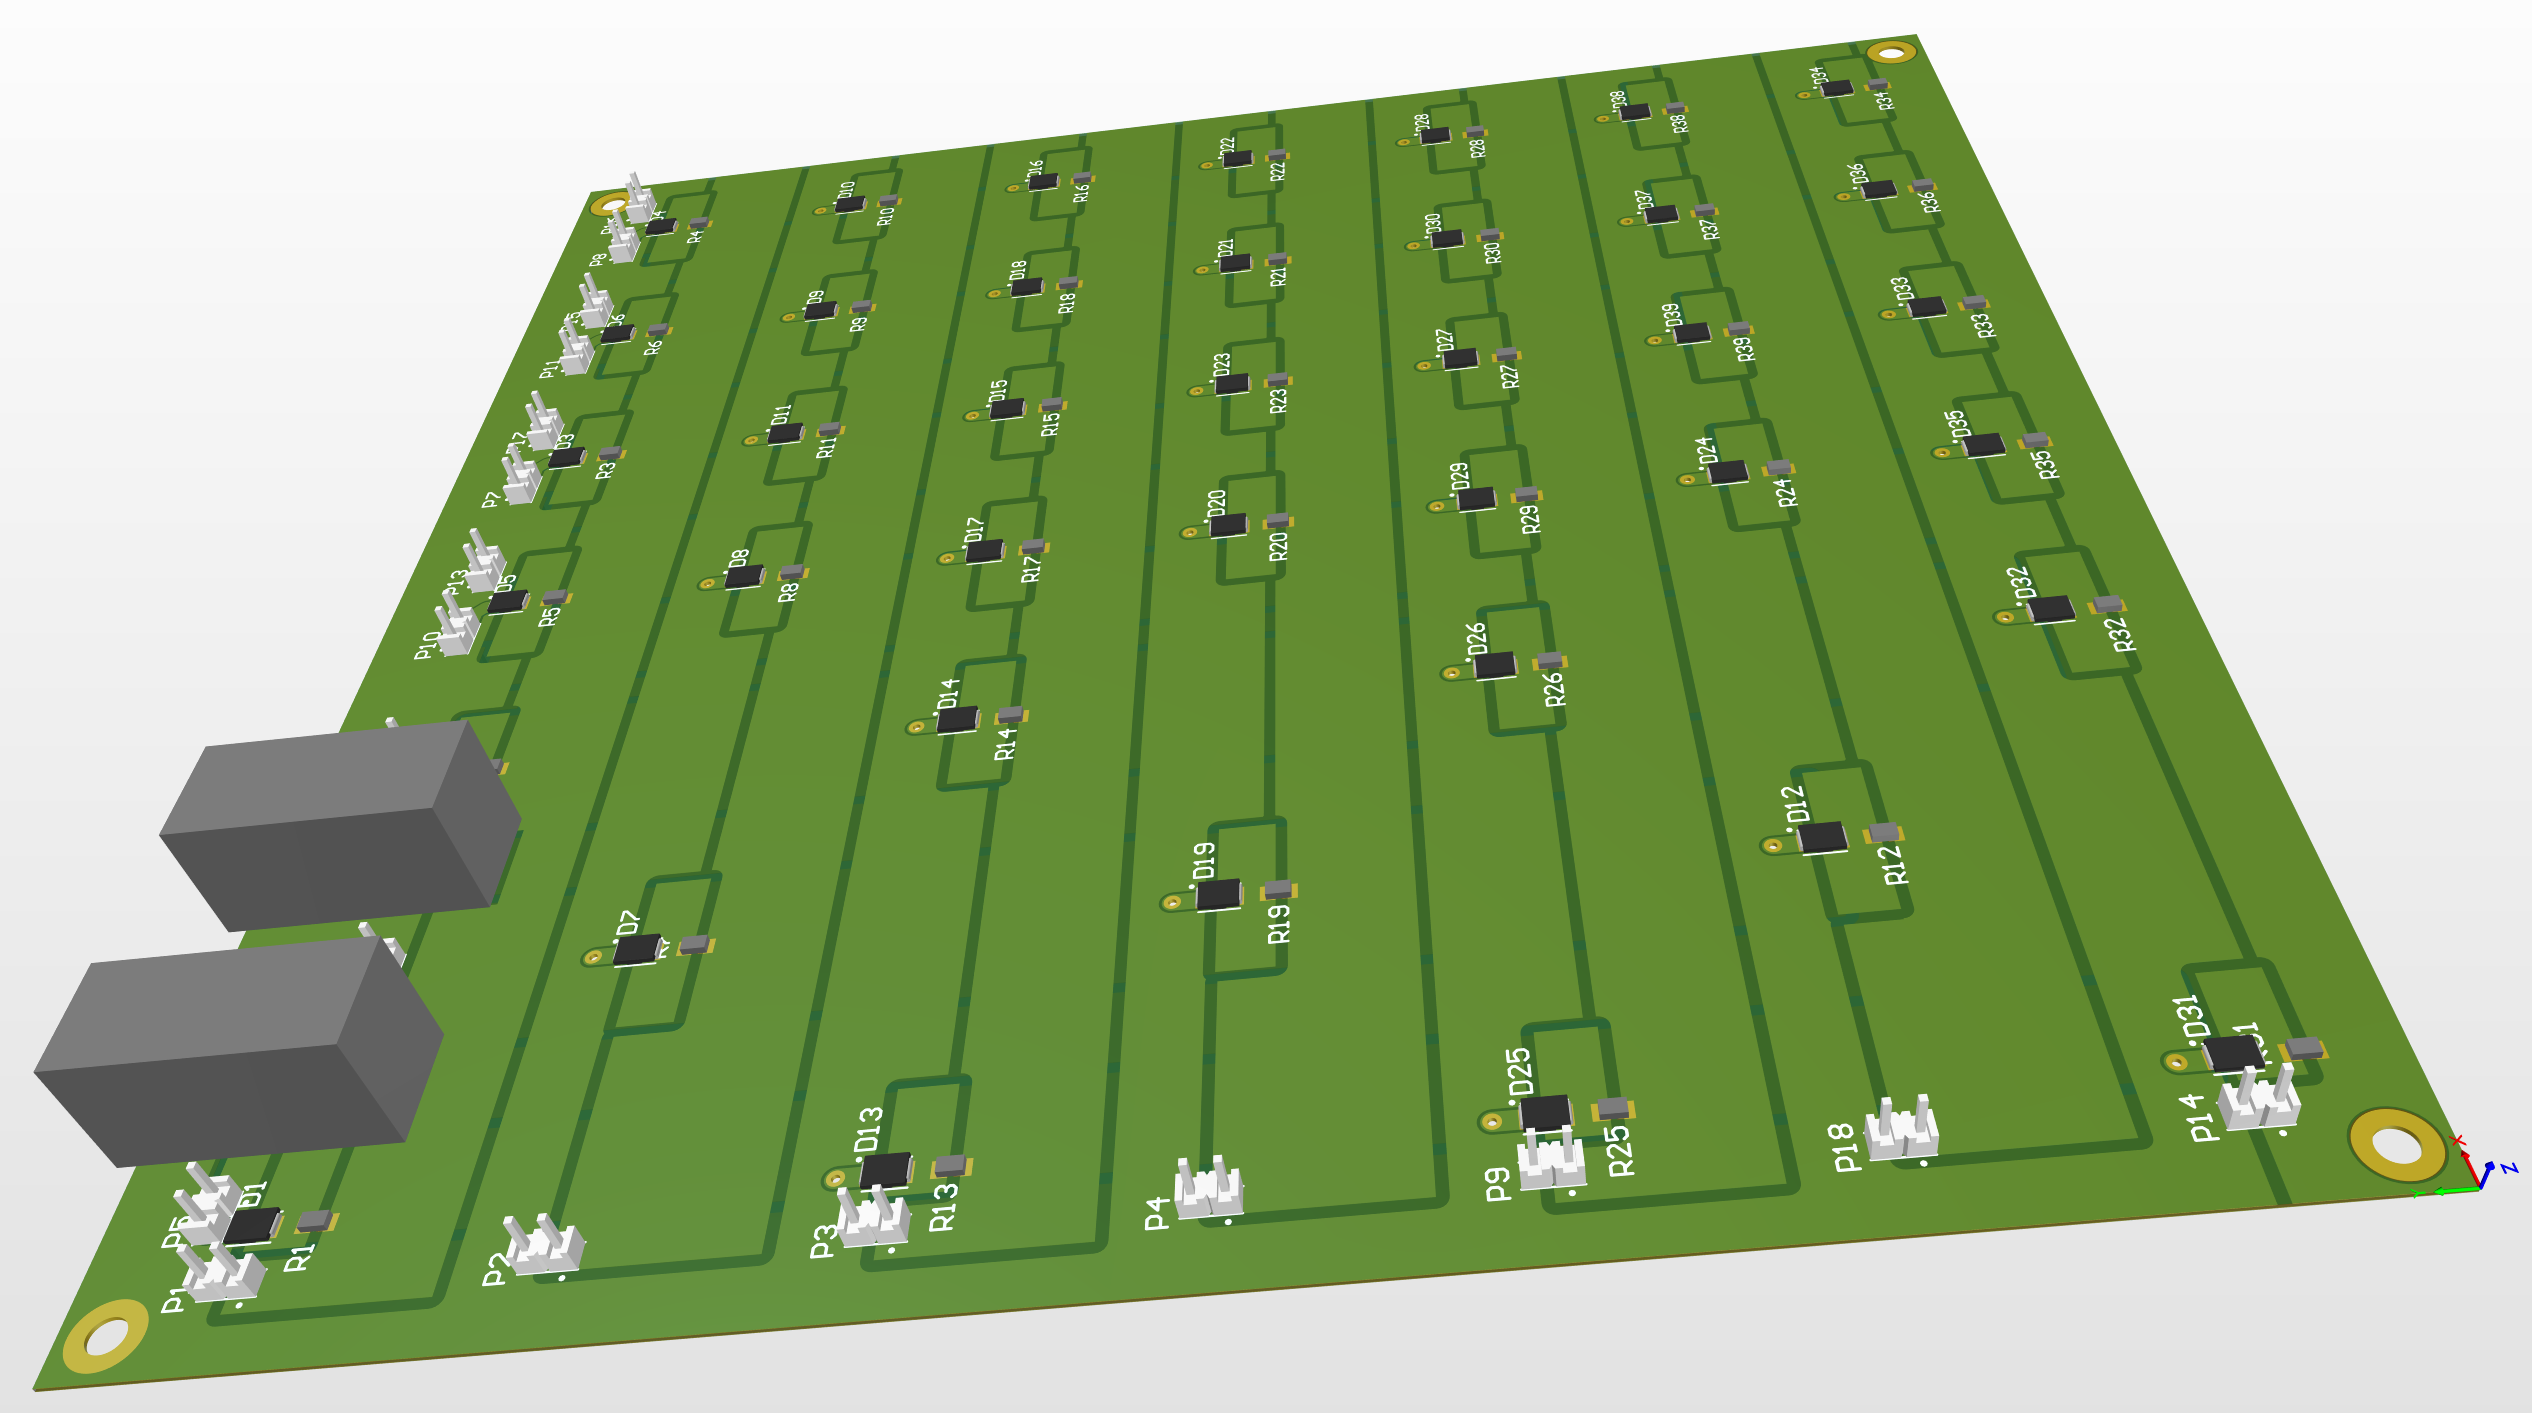
\includegraphics[width=0.9\textwidth]{3-development/images/Backlight.png}
	\caption{3D-Model of the backlight PCB.\label{development:pcb}}
\end{figure} 
The LEDs have been placed less dense in the center, to compensate that the image is generally darker on it's edges.
This is also called vignetting \cite{vignetting}.

To spread the light evenly, a diffusion filter (Kimoto OptSaver 100ST) is mounted in front of the two PCBs.
To inspect how the luminance of the backlight is captured by the camera, different images of the backlight are plotted as a surface- and contour-plot.
Firstly, the empty surface (diffusion filter but no geometry pattern) is analyzed in Figure \ref{development:3d0}. 
\begin{figure}[ht]
	\centering
	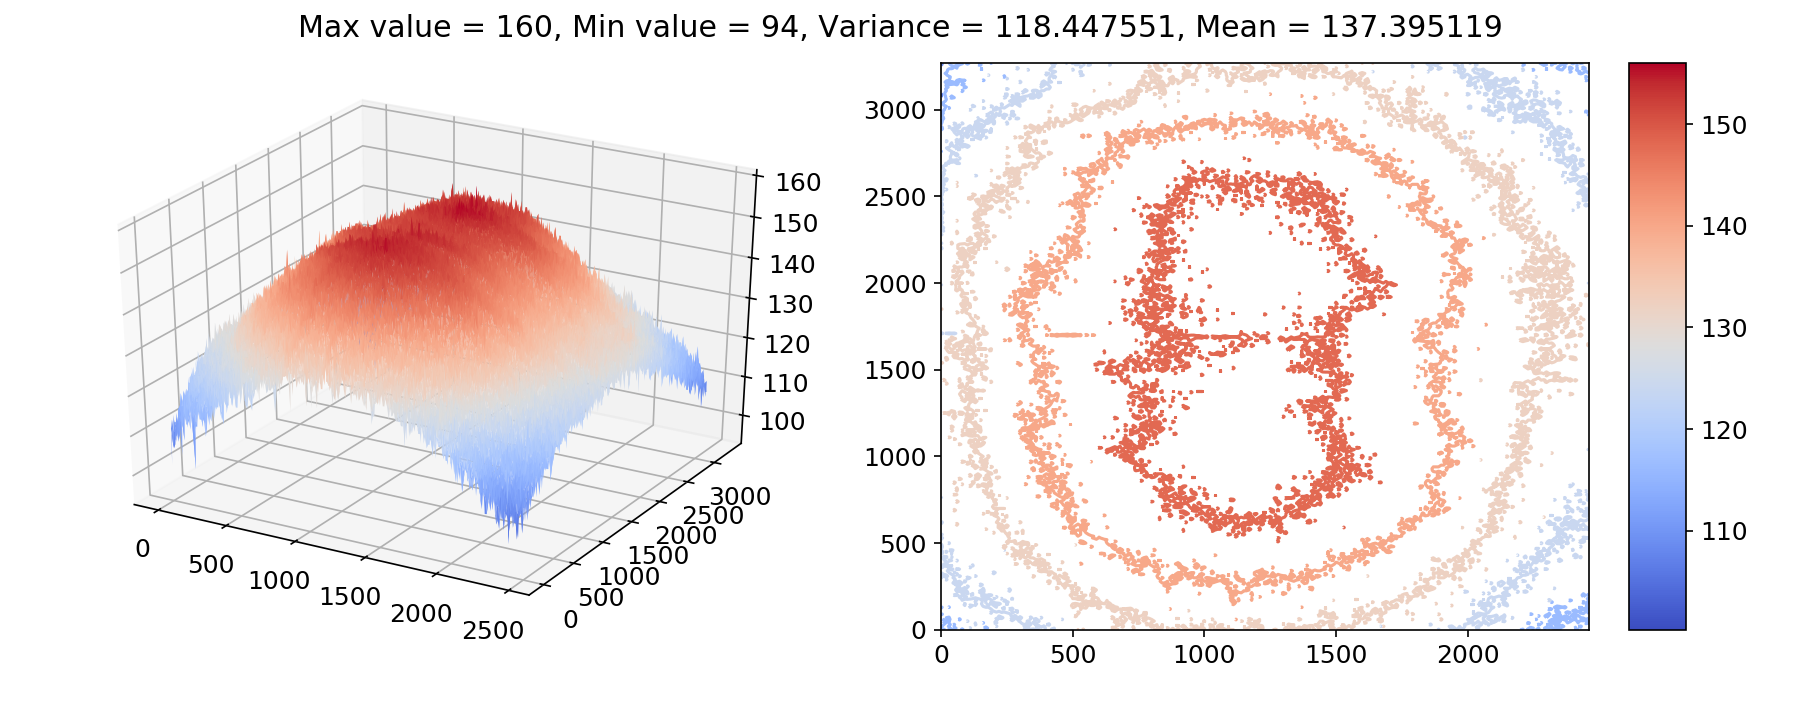
\includegraphics[trim=50 0 0 0,clip,width=0.9\linewidth]{3-development/backlight/3d0.png}
	\caption{Backlight with diffusion filter but no geometry pattern.\label{development:3d0}}
\end{figure} 
In this plot we can spot that our edges are less intense as the middle of our backlight.
With the camera driver regulating our brightness to a mean close to 127, we have a maximum value of 160 and a minimum value of 94.
The image used for the plots in Figure \ref{development:3d1} are taken with the additional geometry pattern on the glass plate.
\begin{figure}[ht]
	\centering
	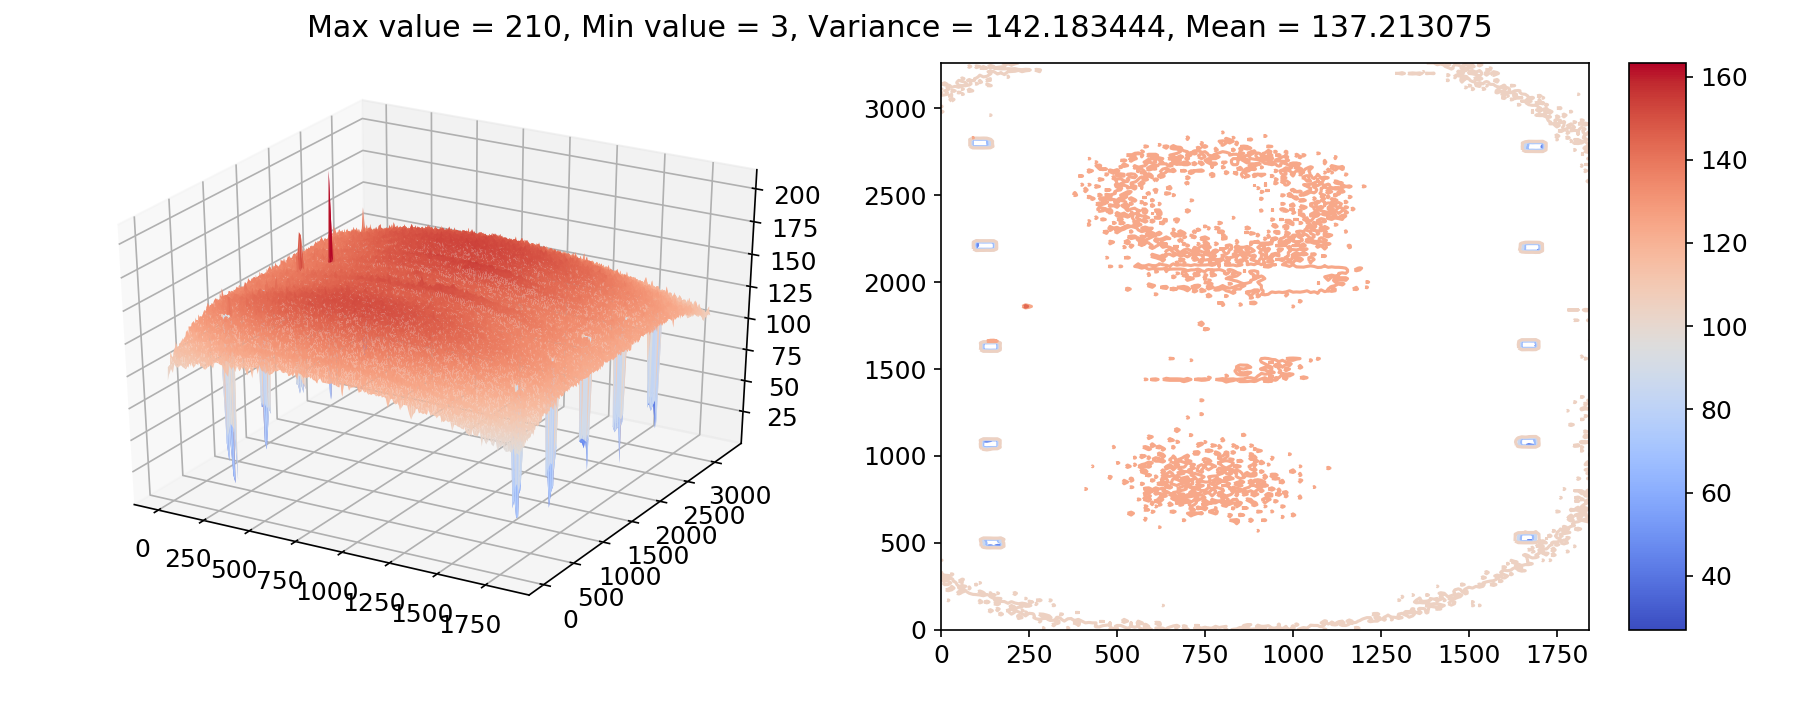
\includegraphics[trim=50 0 0 0,clip,width=0.9\linewidth]{3-development/backlight/3d1.png}
	\caption{Backlight with diffusion filter and geometry pattern.\label{development:3d1}}
\end{figure} 
Now the lowest point lays in the black squares with the value 3.
The maximum value of 210 is an outlier, which can be caused by a reflection or not well positioned diffusion filter.
In the plot in Figure \ref{development:3d4} we can see that the some edges of the spring are very close to the background brightness.
\begin{figure}[ht]
	\centering
	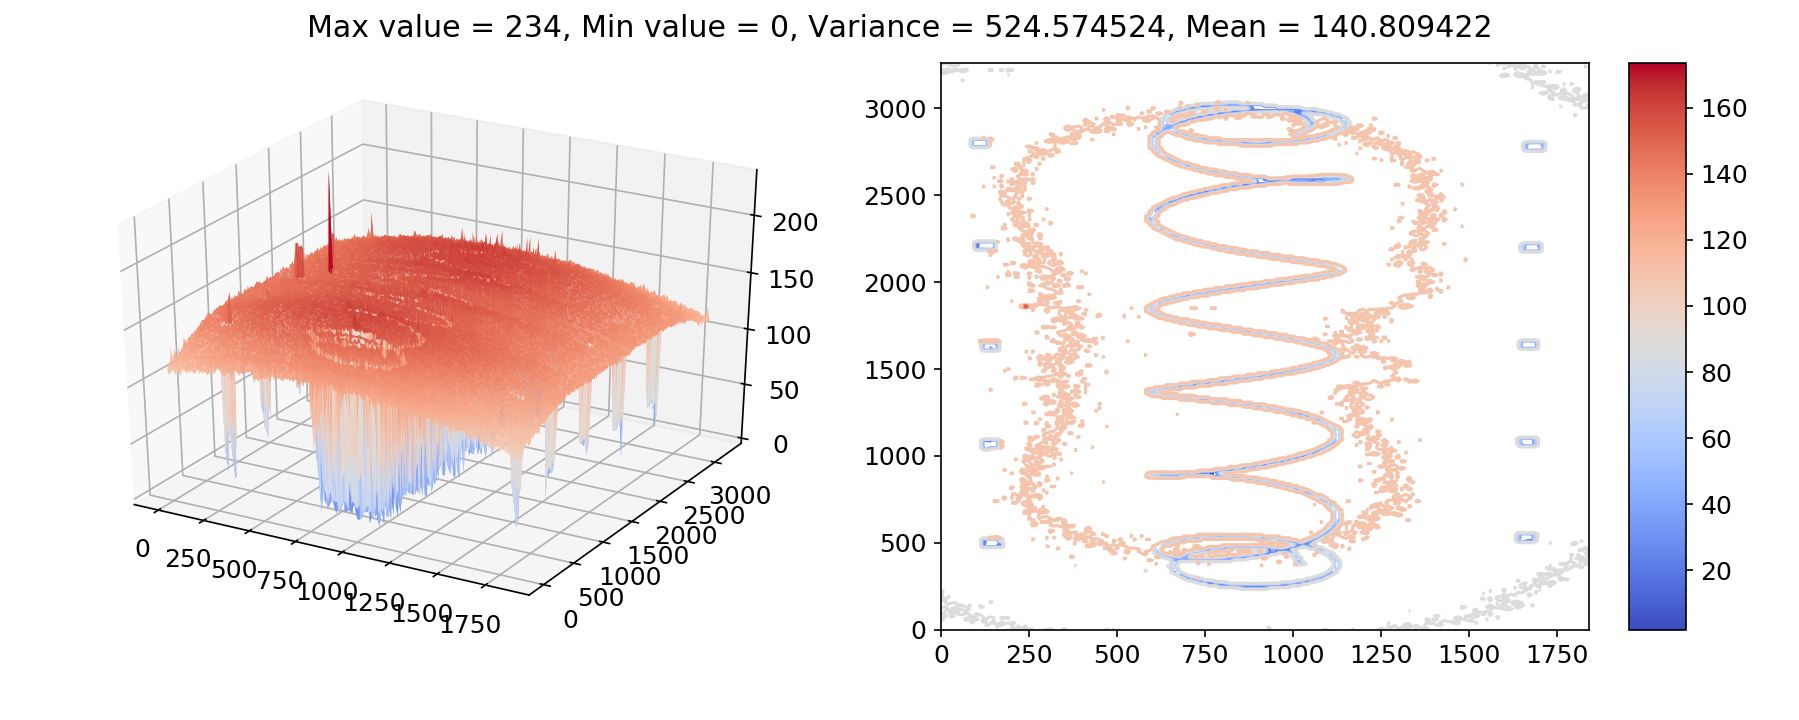
\includegraphics[trim=50 0 0 0,clip,width=0.9\linewidth]{3-development/backlight/3d4.png}
	\caption{Backlight with diffusion filter, geometry pattern and object (spring).\label{development:3d4}}
\end{figure} 
This happens because there is stray light illuminating the edge of the spring.
Since the object is three dimensional, the parts closer to the backlight (on the plane) are illuminated more by stray light than parts further away.

\newpage
\subsection{Demonstrator}
The demonstrator consists of three essential components.
A mechanical construction made out of aluminum profiles, the backlight with the glass plate and the Jetson Nano with the Raspberry Pi camera.  
This construction, as shown in Figure \ref{development:demo}, makes it easy to adjust the distance and position of the parts, while developing the software.
\begin{figure}[ht]
	\centering
	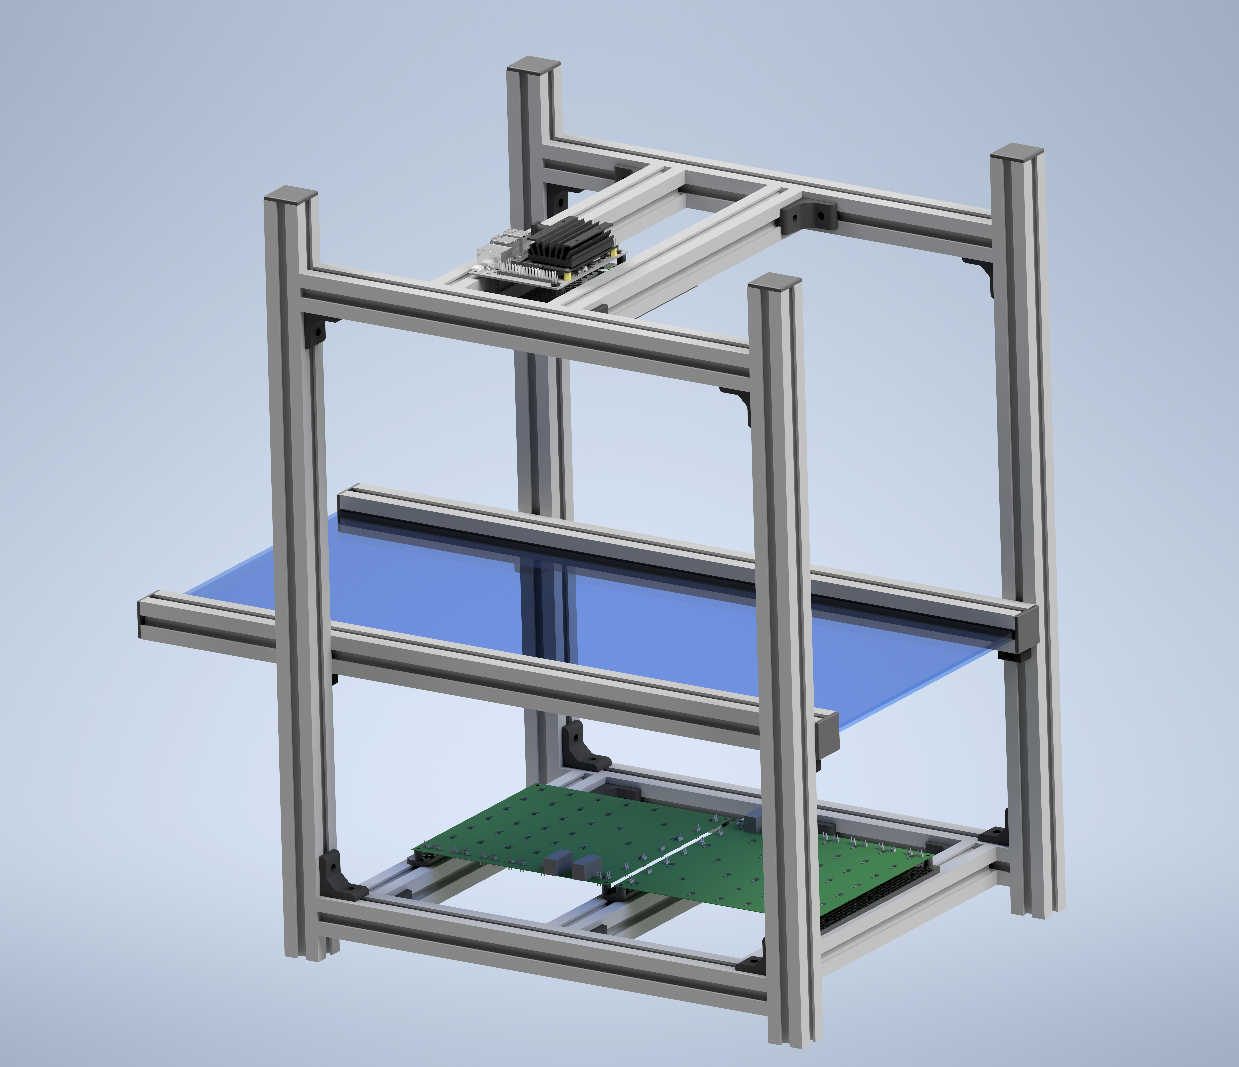
\includegraphics[width=0.9\textwidth]{3-development/images/Demonstrator.png}
	\caption{3D-Model of the demonstrator.\label{development:demo}}
\end{figure} 
The whole construction can be tilted.
This makes it possible to let objects slide through the field of view of the camera, to simulate dynamic measuring.

\newpage
\subsection{Production cost}
Table \ref{development:cost} lists the cost of the Demonstrator.
Note that the price of one PCB drops to 1.35\,CHF if a batch of 2000 is ordered.
\begin{table}[ht]
	\centering
	\begin{tabular}{|l|c|c|c|}
		\hline
		Component & quantity & price per unit (CHF)& total (CHF)\\
		\hline
		Glass & 3 & 10.95 & 32.85\\
		\hline
		Raspberry Pi camera&1&31.90&31.90\\
		\hline
		Jetson Nano developer kit&1&158.40&158.40\\
		\hline	
		Aluminum profiles and accessories&1&437.40&437.40\\
		\hline
		PCB&2&53.06&106.12\\
		\hline
		LED white 76\,lm&78&0.035&2.73\\
		\hline
		Resistor 13\,$\Omega$&78&0.043&3.354\\
		\hline
		Jumper&36&0.037&1.332\\
		\hline
		Socket&4&2.02&8.08\\
		\hline
		\hline
		\textbf{Total}&&&728.168\\
		\hline
	\end{tabular}
	\caption{Demonstrator costs.\label{development:cost}}
\end{table}